\documentclass{standalone}
\usepackage[utf8]{inputenc}
\usepackage{pgfplots}
\DeclareUnicodeCharacter{2212}{−}
\usepgfplotslibrary{groupplots}
\usepgfplotslibrary{dateplot}
\usetikzlibrary{patterns}
\usetikzlibrary{shapes.arrows}
\pgfplotsset{compat=newest}
\begin{document}
% This file was created by tikzplotlib v0.9.1.
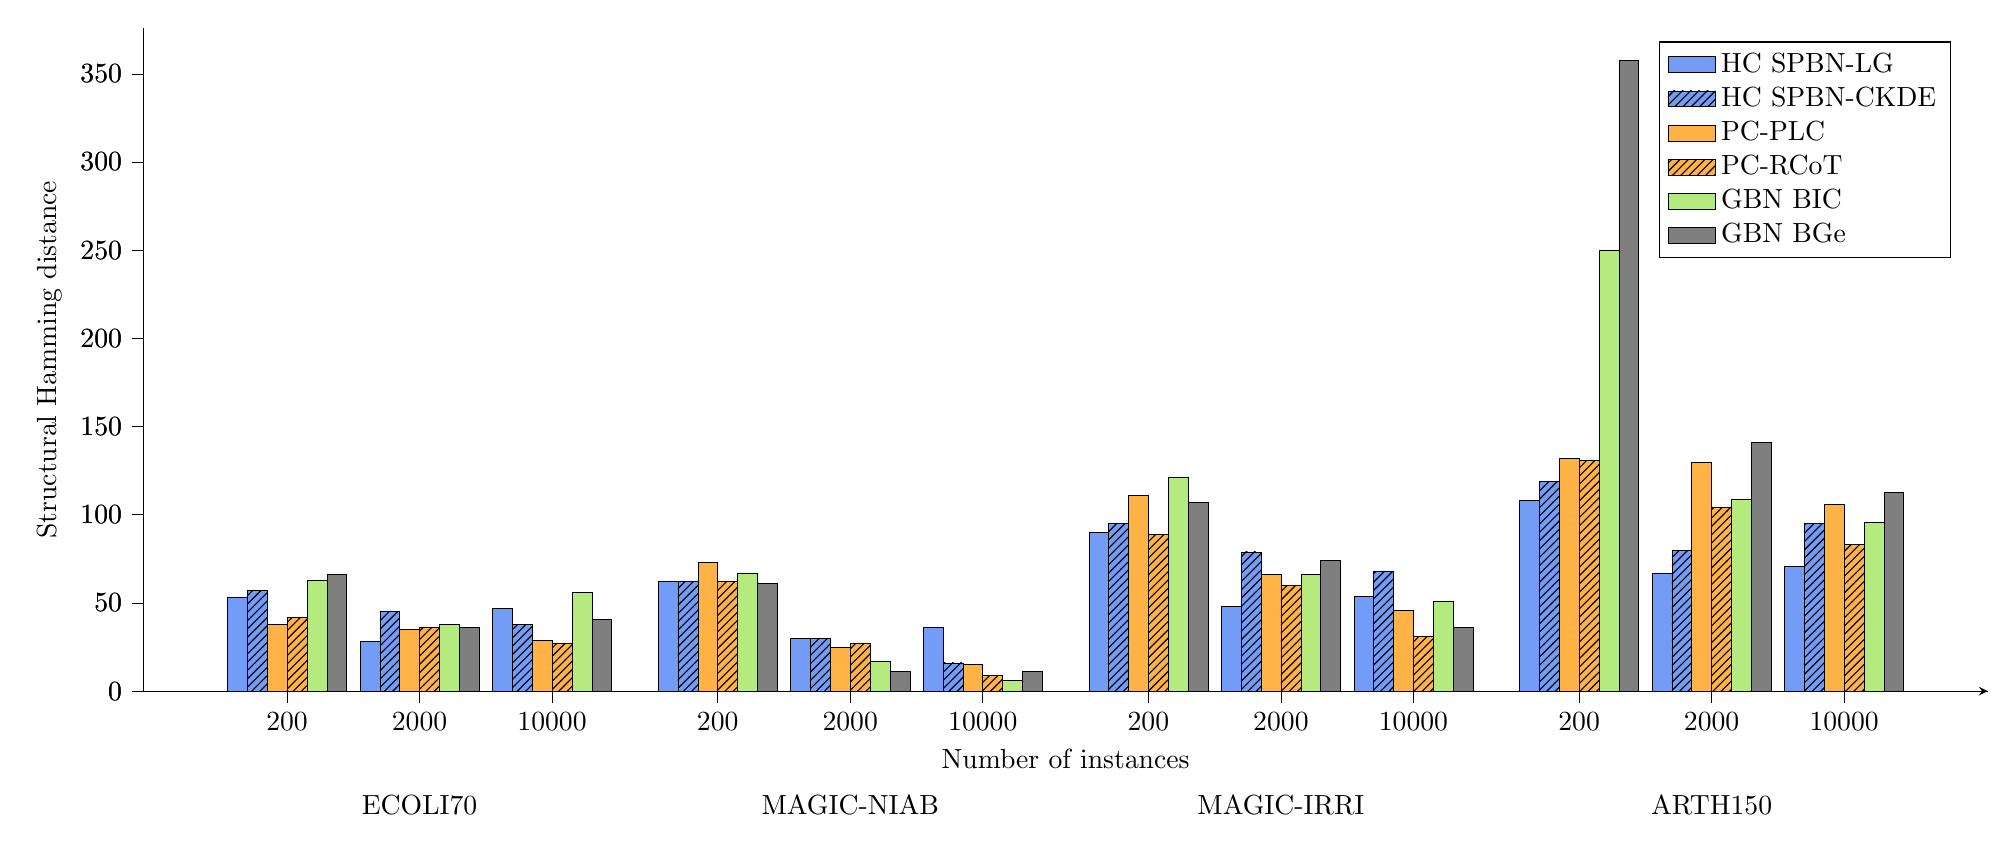
\begin{tikzpicture}

\definecolor{color0}{rgb}{0.447058823529412,0.611764705882353,0.96078431372549}
\definecolor{color1}{rgb}{1,0.701960784313725,0.274509803921569}
\definecolor{color2}{rgb}{0.709803921568627,0.917647058823529,0.498039215686275}

\begin{axis}[
height=10cm,
tick align=outside,
tick pos=left,
width=25cm,
x grid style={white!69.0196078431373!black},
xmin=-0.6325, xmax=13.2825,
xtick style={color=black},
xtick={0.45,1.45,2.45,3.7,4.7,5.7,6.95,7.95,8.95,10.2,11.2,12.2},
xticklabels={200,2000,10000,200,2000,10000,200,2000,10000,200,2000,10000},
y grid style={white!69.0196078431373!black},
ylabel={Structural Hamming distance},
xlabel={Number of instances},
ymin=0, ymax=375.9,
ytick style={color=black},
legend cell align={left},
axis x line*=bottom,
axis y line*=left,
]
\draw[draw=black,fill=color0,very thin] (axis cs:0,0) rectangle (axis cs:0.15,53);
\draw[draw=black,fill=color0,very thin] (axis cs:1,0) rectangle (axis cs:1.15,28);
\draw[draw=black,fill=color0,very thin] (axis cs:2,0) rectangle (axis cs:2.15,47);
\draw[draw=black,fill=color0,very thin] (axis cs:3.25,0) rectangle (axis cs:3.4,62);
\draw[draw=black,fill=color0,very thin] (axis cs:4.25,0) rectangle (axis cs:4.4,30);
\draw[draw=black,fill=color0,very thin] (axis cs:5.25,0) rectangle (axis cs:5.4,36);
\draw[draw=black,fill=color0,very thin] (axis cs:6.5,0) rectangle (axis cs:6.65,90);
\draw[draw=black,fill=color0,very thin] (axis cs:7.5,0) rectangle (axis cs:7.65,48);
\draw[draw=black,fill=color0,very thin] (axis cs:8.5,0) rectangle (axis cs:8.65,54);
\draw[draw=black,fill=color0,very thin] (axis cs:9.75,0) rectangle (axis cs:9.9,108);
\draw[draw=black,fill=color0,very thin] (axis cs:10.75,0) rectangle (axis cs:10.9,67);
\draw[draw=black,fill=color0,very thin] (axis cs:11.75,0) rectangle (axis cs:11.9,71);
\draw[draw=black,fill=color0,very thin,postaction={pattern=north east lines}] (axis cs:0.15,0) rectangle (axis cs:0.3,57);
\draw[draw=black,fill=color0,very thin,postaction={pattern=north east lines}] (axis cs:1.15,0) rectangle (axis cs:1.3,45);
\draw[draw=black,fill=color0,very thin,postaction={pattern=north east lines}] (axis cs:2.15,0) rectangle (axis cs:2.3,38);
\draw[draw=black,fill=color0,very thin,postaction={pattern=north east lines}] (axis cs:3.4,0) rectangle (axis cs:3.55,62);
\draw[draw=black,fill=color0,very thin,postaction={pattern=north east lines}] (axis cs:4.4,0) rectangle (axis cs:4.55,30);
\draw[draw=black,fill=color0,very thin,postaction={pattern=north east lines}] (axis cs:5.4,0) rectangle (axis cs:5.55,16);
\draw[draw=black,fill=color0,very thin,postaction={pattern=north east lines}] (axis cs:6.65,0) rectangle (axis cs:6.8,95);
\draw[draw=black,fill=color0,very thin,postaction={pattern=north east lines}] (axis cs:7.65,0) rectangle (axis cs:7.8,79);
\draw[draw=black,fill=color0,very thin,postaction={pattern=north east lines}] (axis cs:8.65,0) rectangle (axis cs:8.8,68);
\draw[draw=black,fill=color0,very thin,postaction={pattern=north east lines}] (axis cs:9.9,0) rectangle (axis cs:10.05,119);
\draw[draw=black,fill=color0,very thin,postaction={pattern=north east lines}] (axis cs:10.9,0) rectangle (axis cs:11.05,80);
\draw[draw=black,fill=color0,very thin,postaction={pattern=north east lines}] (axis cs:11.9,0) rectangle (axis cs:12.05,95);
\draw[draw=black,fill=color1,very thin] (axis cs:0.3,0) rectangle (axis cs:0.45,38);
\draw[draw=black,fill=color1,very thin] (axis cs:1.3,0) rectangle (axis cs:1.45,35);
\draw[draw=black,fill=color1,very thin] (axis cs:2.3,0) rectangle (axis cs:2.45,29);
\draw[draw=black,fill=color1,very thin] (axis cs:3.55,0) rectangle (axis cs:3.7,73);
\draw[draw=black,fill=color1,very thin] (axis cs:4.55,0) rectangle (axis cs:4.7,25);
\draw[draw=black,fill=color1,very thin] (axis cs:5.55,0) rectangle (axis cs:5.7,15);
\draw[draw=black,fill=color1,very thin] (axis cs:6.8,0) rectangle (axis cs:6.95,111);
\draw[draw=black,fill=color1,very thin] (axis cs:7.8,0) rectangle (axis cs:7.95,66);
\draw[draw=black,fill=color1,very thin] (axis cs:8.8,0) rectangle (axis cs:8.95,46);
\draw[draw=black,fill=color1,very thin] (axis cs:10.05,0) rectangle (axis cs:10.2,132);
\draw[draw=black,fill=color1,very thin] (axis cs:11.05,0) rectangle (axis cs:11.2,130);
\draw[draw=black,fill=color1,very thin] (axis cs:12.05,0) rectangle (axis cs:12.2,106);
\draw[draw=black,fill=color1,very thin,postaction={pattern=north east lines}] (axis cs:0.45,0) rectangle (axis cs:0.6,42);
\draw[draw=black,fill=color1,very thin,postaction={pattern=north east lines}] (axis cs:1.45,0) rectangle (axis cs:1.6,36);
\draw[draw=black,fill=color1,very thin,postaction={pattern=north east lines}] (axis cs:2.45,0) rectangle (axis cs:2.6,27);
\draw[draw=black,fill=color1,very thin,postaction={pattern=north east lines}] (axis cs:3.7,0) rectangle (axis cs:3.85,62);
\draw[draw=black,fill=color1,very thin,postaction={pattern=north east lines}] (axis cs:4.7,0) rectangle (axis cs:4.85,27);
\draw[draw=black,fill=color1,very thin,postaction={pattern=north east lines}] (axis cs:5.7,0) rectangle (axis cs:5.85,9);
\draw[draw=black,fill=color1,very thin,postaction={pattern=north east lines}] (axis cs:6.95,0) rectangle (axis cs:7.1,89);
\draw[draw=black,fill=color1,very thin,postaction={pattern=north east lines}] (axis cs:7.95,0) rectangle (axis cs:8.1,60);
\draw[draw=black,fill=color1,very thin,postaction={pattern=north east lines}] (axis cs:8.95,0) rectangle (axis cs:9.1,31);
\draw[draw=black,fill=color1,very thin,postaction={pattern=north east lines}] (axis cs:10.2,0) rectangle (axis cs:10.35,131);
\draw[draw=black,fill=color1,very thin,postaction={pattern=north east lines}] (axis cs:11.2,0) rectangle (axis cs:11.35,104);
\draw[draw=black,fill=color1,very thin,postaction={pattern=north east lines}] (axis cs:12.2,0) rectangle (axis cs:12.35,83);
\draw[draw=black,fill=color2,very thin] (axis cs:0.6,0) rectangle (axis cs:0.75,63);
\draw[draw=black,fill=color2,very thin] (axis cs:1.6,0) rectangle (axis cs:1.75,38);
\draw[draw=black,fill=color2,very thin] (axis cs:2.6,0) rectangle (axis cs:2.75,56);
\draw[draw=black,fill=color2,very thin] (axis cs:3.85,0) rectangle (axis cs:4,67);
\draw[draw=black,fill=color2,very thin] (axis cs:4.85,0) rectangle (axis cs:5,17);
\draw[draw=black,fill=color2,very thin] (axis cs:5.85,0) rectangle (axis cs:6,6);
\draw[draw=black,fill=color2,very thin] (axis cs:7.1,0) rectangle (axis cs:7.25,121);
\draw[draw=black,fill=color2,very thin] (axis cs:8.1,0) rectangle (axis cs:8.25,66);
\draw[draw=black,fill=color2,very thin] (axis cs:9.1,0) rectangle (axis cs:9.25,51);
\draw[draw=black,fill=color2,very thin] (axis cs:10.35,0) rectangle (axis cs:10.5,250);
\draw[draw=black,fill=color2,very thin] (axis cs:11.35,0) rectangle (axis cs:11.5,109);
\draw[draw=black,fill=color2,very thin] (axis cs:12.35,0) rectangle (axis cs:12.5,96);
\draw[draw=black,fill=black,fill opacity=0.501960784313725,very thin] (axis cs:0.75,0) rectangle (axis cs:0.9,66);
\draw[draw=black,fill=black,fill opacity=0.501960784313725,very thin] (axis cs:1.75,0) rectangle (axis cs:1.9,36);
\draw[draw=black,fill=black,fill opacity=0.501960784313725,very thin] (axis cs:2.75,0) rectangle (axis cs:2.9,41);
\draw[draw=black,fill=black,fill opacity=0.501960784313725,very thin] (axis cs:4,0) rectangle (axis cs:4.15,61);
\draw[draw=black,fill=black,fill opacity=0.501960784313725,very thin] (axis cs:5,0) rectangle (axis cs:5.15,11);
\draw[draw=black,fill=black,fill opacity=0.501960784313725,very thin] (axis cs:6,0) rectangle (axis cs:6.15,11);
\draw[draw=black,fill=black,fill opacity=0.501960784313725,very thin] (axis cs:7.25,0) rectangle (axis cs:7.4,107);
\draw[draw=black,fill=black,fill opacity=0.501960784313725,very thin] (axis cs:8.25,0) rectangle (axis cs:8.4,74);
\draw[draw=black,fill=black,fill opacity=0.501960784313725,very thin] (axis cs:9.25,0) rectangle (axis cs:9.4,36);
\draw[draw=black,fill=black,fill opacity=0.501960784313725,very thin] (axis cs:10.5,0) rectangle (axis cs:10.65,358);
\draw[draw=black,fill=black,fill opacity=0.501960784313725,very thin] (axis cs:11.5,0) rectangle (axis cs:11.65,141);
\draw[draw=black,fill=black,fill opacity=0.501960784313725,very thin] (axis cs:12.5,0) rectangle (axis cs:12.65,113);
\addlegendimage{area legend,draw=black,fill=color0,very thin}
\addlegendimage{area legend,draw=black,fill=color0,very thin,postaction={pattern=north east lines}}
\addlegendimage{area legend,draw=black,fill=color1,very thin}
\addlegendimage{area legend,draw=black,fill=color1,very thin,postaction={pattern=north east lines}}
\addlegendimage{area legend,draw=black,fill=color2,very thin}
\addlegendimage{area legend,draw=black,fill=black,fill opacity=0.501960784313725,very thin}

\legend{HC SPBN-LG,HC SPBN-CKDE,PC-PLC,PC-RCoT,GBN BIC,GBN BGe}
\end{axis}

\begin{axis}[
axis x line=top,
height=10cm,
tick align=outside,
tick pos=left,
width=25cm,
x grid style={white!69.0196078431373!black},
xmin=-0.6325, xmax=13.2825,
xtick style={color=black},
xtick={1.45,4.7,7.95,11.2},
xticklabels={ECOLI70,MAGIC-NIAB,MAGIC-IRRI,ARTH150},
y grid style={white!69.0196078431373!black},
ymin=0, ymax=375.9,
ytick style={color=black},
x tick label style={yshift={-3em}},
axis x line*=bottom,
axis y line*=left,
]
\end{axis}

\end{tikzpicture}

\end{document}
